\chapter{Architecture}

\minitoc

The system is to be described in this chapter. This includes the main parts of the system, the architectural drivers, how they are connected together, and their collaboration. The architecture will be described through the 4+1 view model. The party members, or the stakeholders of the system, will have different concerns, so the 4+1 view model will help us describe the system for each of them, and make sure that all expectations are accounted for.  

First section presents the Architectural Drivers \ref{Architectural drivers} which are the main implications that can affect our system. Second section, Stakeholders \ref{Stakeholders}, lists the stakeholders involved in the development of this system as well as their concerns. Third section, the Views \ref{Views}, helps capturing the whole architecture for the different stakeholders to understand. Fourth section, Architectural Tactics \ref{Tactics}, is used to show how the goals of the system will be reached. Fifth section, Architectural patterns \ref{Architectural patterns}, will show how the architectural tactics will be supported.

\clearpage


\section{Architectural drivers} \label{Architectural drivers}
The architectural drivers defines the project and its scope. 

\begin{itemize}
    \item Improving the efficiency in the chosen domain - The traditional web application system is to be improved efficiency-wise, so power users will be able to use less time on more tasks. (non-functional requirement)
    \item Proving the concept in general - Our solution should be applicable to more general problems than those described by the chosen domain. (business constraint)
    \item Minimum console functionality - The system's console should have capabilities on par with a traditional web application: Creating objects, editing objects, deleting objects, working with lists of objects.  (functional requirement)
    \item Added flexibility - The console should allow the user to perform tasks that are not possible with a web application of comparable complexity and development cost. (non-functional requirement)
    \item Console in a web context - The console should operate in a web browser environment. (technical constraint)
    \item Tolerate changes in requirements - We must use an approach that tolerates iterative changes to the demands from the customer. If new functionality is proposed and deemed likely to make the prototype more useful, it should be implemented asap. (business constraint)
    \item Delivery on time - The project must be finished on a fixed schedule. (business constraint) 
    \item Academically sound process - The project should be executed using methods that satisfy the academical context. (business constraint)
\end{itemize}


\section{Stakeholders} \label{Stakeholders}
The stakeholders and their concerns when it comes to the system.

\begin{itemize}
    \item Developer
    \begin{itemize}
        \item Deadline, the system should be done by the deadline
        \item Solve the problem and deliver a system the customer will be satisfied with.
        \item Learn new technologies
        \item Get experience with project management
        \end{itemize}
    \item Customer
    \begin{itemize}
        \item Gets a working system, which satisfies the customers wants
        \item Get a usable report on the concept, which satisfies the customers wants
    \end{itemize}
    \item End user
    \begin{itemize}
        \item Improve efficiency
        \item Easy to use after some training
    \end{itemize}
\end{itemize}



\section{Views} \label{Views}
The 4+1 view model\cite{Kruchten}. Here the views will be described, and how they will look in our architecture. This approach of designing makes the system easier to understand for both the developer, user and the customer, and gives the developers a good overview of what need to be done. Diagrams are based on Martin Fowler's UML\cite{Fowl04}

\subsection{Logical View}
Describes the functionality in the system from the end users perspective. The end users will mainly be a power users, wanting to perform object editing tasks efficiently. This view will be described through class diagrams.  We had some bigger changes from sprint two to three. The development of the logical view, and the road taken to reach this functionality representation can be observed through the sprint chapters.

\begin{figure}[h]
\centering
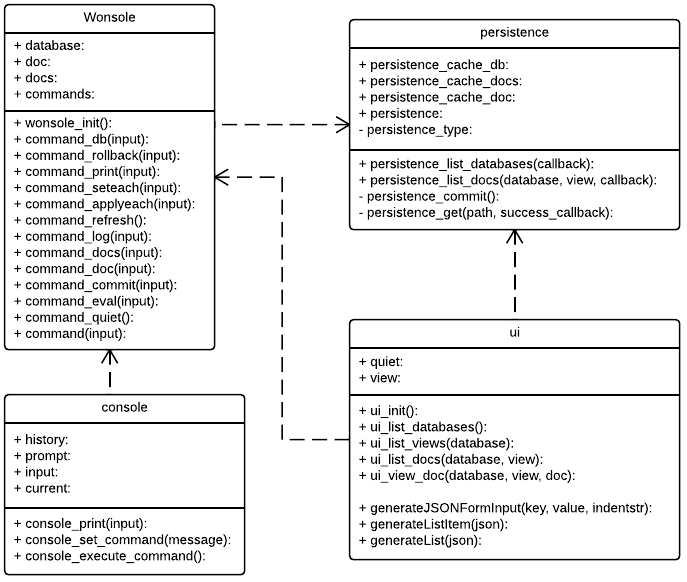
\includegraphics[width=6in]{image/architecture/clientClassDiagram.png}
\caption{Client Class Diagram}
\label{figure:clientClassDiagram}
\end{figure}

Figure~\ref{figure:clientClassDiagram} The client class diagram gives an overview of the class structure of system, and how the classes collaborate. The Wonsole class possesses the commands used by the console to run different actions. Depending on the command, the console's input will lead to an action. This can change the objects in memory, fetch objects from the server, and more. The ui class represent these objects in a readable fashion, and actions to the objects can also here be done. The persistence class lets the user fetch and store objects to the server.

\begin{figure}[h]
\centering
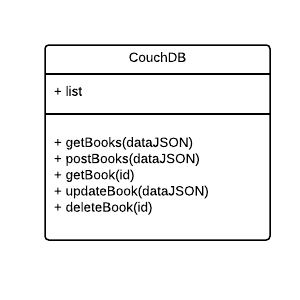
\includegraphics[width=2in]{image/architecture/serverClassDiagram.png}
\caption{Client Class Diagram}
\label{figure:serverClassDiagram}
\end{figure}

Figure~\ref{figure:serverClassDiagram} The server class diagram shows how the REST api is set up. Since the CouchDB in an integrated REST and server system we only have one class here, which can easily communicate with the server.

\subsection{Physical View}
Describes the system from the system engineer's perspective. And explains the physical connections between the software components. Can help to show how changes affect different physical parts of the system, and their impact. Described through a deployment diagram. 

\begin{figure}[h]
\centering
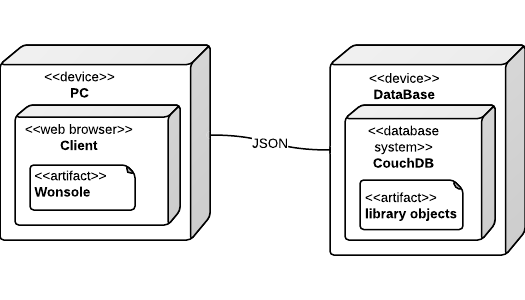
\includegraphics[width=4in]{image/architecture/DeploymentDiagram.png}
\caption{Deployment Diagram}
\label{figure:DeploymentDiagram}
\end{figure}

Figure~\ref{figure:DeploymentDiagram} The structure of the system is divided into two different parts. Here we can see the client can be run on its own computer, and will communicate with the server through JSON. The server is of the type CouchDB and holds the objects for the client to retrieve when wanted.  


\subsection{Development View}
Describes the system from the programmer's perspective. This will be described through how the different component parts are separated. Can help dividing the system into smaller parts, which can easily be developed. Component and package diagrams will show this.

\begin{figure}[h]
\centering
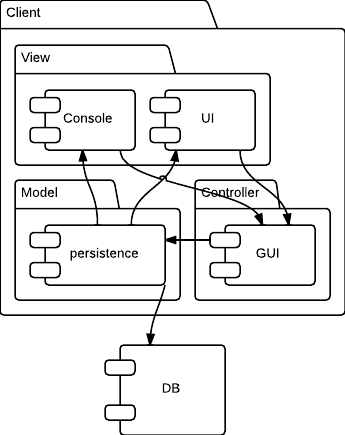
\includegraphics[width=3in]{image/architecture/ComponentDiagram.png}
\caption{Component Diagram}
\label{figure:ComponentDiagram}
\end{figure}

Figure~\ref{figure:ComponentDiagram} These components form a three layered structure. Where the front end (the client) is the upper layer. This layer communicates with the server through the second layer.


\subsection{Scenarios}
Is the + 1 in the 4 + 1 view model. It describes the system through a set of use cases/scenarios. These use cases/scenarios describes how the objects and processes work together. The scenarios can be found in Chapter 4, Requirements.


\section{Architectural tactics} \label{Tactics}
The architectural tactics are used to describe how different qualities of the system are achieved. 

\subsection{Modifiability}
\subsubsection{Anticipate changes}
Probable changes should be anticipated, and accounted for, so extending the system with new functionality should be possible. This is important since we are dealing with a prototype/proof of concept system. So the customer might change the direction we are going in through out the project, this will lead to changes, and the architecture should be able to bend after these new inputs. 

This can be handled with a well defined functionality map, so that the expected system functionalities are accounted for when the system is constructed. 

\subsubsection{Ripple-effect prevention}
It will also be important to make sure that too much does not depend on too much, so it will be possible to avoid potential ripple effects. This happens when one change can expand into the need of changing everything. 

This can be prevented by encapsulating information, or constructing interfaces and maintain existing interfaces. 


\section{Architectural patterns} \label{Architectural patterns}
The patterns can help solve different kinds of problems with known solutions used before on similar problems.

\subsection{Multi-tier}
The architecture of the system will be of the multi-tier kind. This means that the presentation, application processing and data management functions will be separated logically. The application (console) will translate the task of the end user, and will be sent to the server through the logical tier.

The console - Translate the task of the end user.
The logical tier - Will receive the translated task from the console, and fetch information from the data storage specified by the console, and set it back to the user.
The data storage - The last tier, and it will contain the information from the library.

\subsubsection{Front end}
The frontend is implemented using JavaScript and HTML. This is the presentation tier, and will let the user interact with the objects desired. The JavaScript performs operation and communicates with the server through AJAX calls. 

\subsubsection{Middle Layer}
The middle layer (Logical tier) is responsible for communication between the server and the client. Since the database is schemeless, most objects are allowed to be sent to the backend, so this layer does not do big logical operations.

\subsubsection{Backend}
This layer (the data tier) stores the information in a database. This information can be sent back through the middle layer to the client on request from the client. 


\subsection{Model-View-Controller}
MVC lets us divide the system into three main parts, the model, the view and the controller. The model is the data structure within the application. The controller is the interface provided for the client to do operations. The view will render the model to the client. 
The client gui and console communication. Since the action made in the console should be reflected in the gui and vice versa, is it natural to use a model-view-controller pattern. The information in the model will then be separated from the view (the display) and the controller which performs an update on the model. 


\subsection{Rationale} \label{Rationale}
Our architecture is greatly affected by the fact that this project is a prototype project, and that we need to be flexible and able adapt to changes from the outside. This means that we should expect possible changes, and prepare for that. Therefore the modifiability is the tactic we focus on.

MVC was a natural choice for model distribution, so the changes done in the console, could be reflected onto the ui and vice versa. 
